\documentclass[11pt,a4paper]{article}

% ---- Encoding & fonts ----
\usepackage[utf8]{inputenc}
\usepackage[T1]{fontenc}
\usepackage{lmodern}

% ---- Math ----
\usepackage{amsmath,amssymb,amsthm}
\usepackage{mathtools}

% ---- Layout ----
\usepackage[margin=2.3cm]{geometry}
\usepackage{enumitem}
\usepackage{booktabs}
\usepackage{array}

% ---- Visuals ----
\usepackage{xcolor}
\usepackage[most]{tcolorbox}
\usepackage{tikz}
\usetikzlibrary{arrows.meta,positioning,calc,fit,backgrounds,shapes.misc}
\usepackage{pgfplots}
\pgfplotsset{compat=1.18}
\usepackage{hyperref}
\hypersetup{colorlinks=true,linkcolor=blue!55!black,urlcolor=blue!55!black}

% ---- Palette (Armenian flag colours for 3-series plots) ----
\definecolor{armRed}{HTML}{D90012}
\definecolor{armBlue}{HTML}{0033A0}
\definecolor{armOrange}{HTML}{F2A800}
\definecolor{ink}{HTML}{22303C}

\setlength{\parindent}{0pt}
\setlength{\parskip}{5pt}

% ---- Boxes ----
\newtcolorbox{problembox}[1][]{enhanced, breakable, sharp corners=south,
  colback=armOrange!10, colframe=armOrange!75!black, boxrule=0.8pt, arc=2mm,
  fonttitle=\bfseries\color{white}, coltitle=white,
  attach boxed title to top left={xshift=4mm,yshift=-2.4mm},
  boxed title style={colback=armOrange!85!black, arc=1mm},
  title={Problem #1}}

\newtcolorbox{ideabox}{enhanced, breakable,
  colback=armBlue!6, colframe=armBlue!70!black, boxrule=0.8pt, arc=2mm,
  fonttitle=\bfseries\color{white}, coltitle=white,
  attach boxed title to top left={xshift=4mm,yshift=-2.4mm},
  boxed title style={colback=armBlue!75!black, arc=1mm},
  title={The idea}}

\newtcolorbox{methodbox}{enhanced, breakable,
  colback=gray!8, colframe=gray!55!black, boxrule=0.7pt, arc=2mm,
  fonttitle=\bfseries, title={$\bigstar$\ Method to remember}}

\newtcolorbox{answerbox}{enhanced, sharp corners=south,
  colback=green!8, colframe=green!50!black, boxrule=1pt, arc=2mm, left=4mm,right=4mm}

\newcommand{\answer}[1]{\begin{answerbox}\centering\textbf{Answer:}\quad #1\end{answerbox}}

% ---- Title ----
\title{\vspace{-1.2cm}\textbf{Discrete Mathematics - Practical 8}\\[2pt]
\large Recurrence Relations: worked solutions\\[2pt]
\normalsize\itshape with the reasoning spelled out, step by step}
\author{}
\date{}

\begin{document}
\maketitle
\vspace{-1.0cm}

% =====================================================================
\section*{Warm-up: what is a recurrence, and what are we asked to do?}

A \textbf{recurrence relation} defines a sequence by expressing each term through
\emph{earlier} terms, together with a few \textbf{initial conditions}. For example
$a_{n}=a_{n-1}+a_{n-2}$ with $a_0=a_1=1$ is the Fibonacci rule.

Two very different tasks appear in this practical, and the two problems below are
exactly one of each:

\begin{itemize}[leftmargin=1.4em,itemsep=2pt]
  \item \textbf{Solve} a recurrence - find a \emph{closed formula} for $a_n$ that does
        not refer to earlier terms (Problem 2). The tool is the
        \emph{characteristic equation}.
  \item \textbf{Build} a recurrence - translate a \emph{counting} question into a
        recurrence, then run it (Problem 6). The tool is a clever \emph{case split}.
\end{itemize}

% =====================================================================
\section*{Problem 2 - Solving a linear recurrence}

\begin{problembox}[2]
Solve the recurrence relation
\[
a_n = 5a_{n-1} - 6a_{n-2},\qquad n>2,
\]
with initial conditions $a_1=2,\ a_2=10$. (\textquotedbl{}Solve\textquotedbl{} $=$ find a closed formula for $a_n$.)
\end{problembox}

\begin{ideabox}
First, name the structure. This recurrence is \textbf{linear} (each $a_i$ appears to the
first power, never $a_i^2$ or $a_ia_j$), \textbf{homogeneous} (nothing is added on the
right), and has \textbf{constant coefficients} ($5$ and $-6$ never change with $n$). For
exactly this kind of recurrence the right guess is a geometric sequence $a_n=r^n$. It is
\emph{not} pulled from a hat; three observations force it.

\textbf{(i) The simplest recurrence is already geometric.} A one-step rule $a_n=b\,a_{n-1}$
multiplies by the same constant $b$ at every step, so
\[
a_n=b\,a_{n-1}=b^2a_{n-2}=\cdots=a_0\,b^{\,n}.
\]
A fixed multiplier applied over and over \emph{is} geometric growth. Our two-step rule is
just two such growths blended together, so we expect geometric pieces.

\textbf{(ii) Geometric is the one shape where stepping back means scaling by a constant.}
If $a_n=r^n$, then $a_{n-1}=\tfrac1r\,a_n$ and $a_{n-2}=\tfrac1{r^2}\,a_n$. A
constant-coefficient recurrence does precisely this: it ties a term to its earlier
neighbours through fixed numbers. The geometric sequence is built to fit that move.

\textbf{(iii) It collapses infinitely many equations into one.} The recurrence must hold
for \emph{every} $n$ at once, which is infinitely many demands. Feed in $a_n=r^n$ and every term
shares the factor $r^{\,n-2}$; cancel it and the index $n$ disappears entirely, leaving the
single equation $r^2=5r-6$. So one well-chosen number $r$ satisfies the rule at step $3$,
step $4$, step $100$, and onward, simultaneously. \emph{That} is the real reason the guess
works: the geometric shape is the only one that makes a constant-coefficient recurrence say
the very same thing at every step. The values of $r$ that fit are the growth rates hidden
inside the recurrence.
\end{ideabox}

\textbf{Step 1 - Substitute the guess.}
Put $a_n=r^n$ into $a_n=5a_{n-1}-6a_{n-2}$:
\[
r^n = 5r^{\,n-1} - 6r^{\,n-2}.
\]
Divide by the smallest power $r^{\,n-2}$ (allowed since $r=0$ only gives the trivial
sequence):
\[
r^2 = 5r - 6 \quad\Longleftrightarrow\quad \boxed{\,r^2 - 5r + 6 = 0\,}.
\]
This is the \textbf{characteristic equation}.

\textbf{Step 2 - Solve it.}
\[
r^2-5r+6=(r-2)(r-3)=0 \quad\Longrightarrow\quad r_1=2,\quad r_2=3.
\]
We found \emph{two} different geometric solutions: $2^n$ and $3^n$.

\textbf{Step 3 - Combine them (superposition).}
Because the recurrence is linear and homogeneous, \emph{any} combination of solutions is
again a solution. With two distinct roots the general solution is
\[
a_n = C\cdot 2^n + D\cdot 3^n,
\]
where $C,D$ are constants. We have exactly two unknowns to match our two initial
conditions, and that is no coincidence.

\textbf{Why is $C\cdot2^n+D\cdot3^n$ \emph{every} solution, not just some of them?} Suppose another
sequence also obeys $a_n=5a_{n-1}-6a_{n-2}$ and happens to agree with our formula at two
consecutive indices. Then they must agree \emph{everywhere}: each next term is forced by the
previous two (and the rule runs backwards as well, fixing the earlier terms). So a solution is
pinned down completely by any two consecutive values, and the constants $C,D$ give exactly
enough freedom to match $a_1$ and $a_2$. Once they are set, the formula \emph{is} the sequence.

\textbf{Step 4 - Use the initial conditions.}
\[
\begin{cases}
a_1=2: & 2C+3D=2,\\[2pt]
a_2=10: & 4C+9D=10.
\end{cases}
\]
Multiply the first equation by $2$ and subtract from the second:
\[
(4C+9D)-(4C+6D)=10-4 \;\Longrightarrow\; 3D=6 \;\Longrightarrow\; D=2,
\]
and then $2C+3(2)=2\Rightarrow C=-2$.

\textbf{Step 5 - Write the closed formula.}
\[
a_n=-2\cdot 2^n+2\cdot 3^n = 2\cdot 3^n - 2^{\,n+1}.
\]

\textbf{Step 6 - Always check.}
\[
a_1=2\cdot3-2^2=6-4=2\ \checkmark\qquad
a_2=2\cdot9-2^3=18-8=10\ \checkmark
\]
\[
a_3 \stackrel{\text{formula}}{=} 2\cdot27-2^4=38
\quad\text{vs}\quad
a_3 \stackrel{\text{recurrence}}{=} 5\cdot10-6\cdot2=38\ \checkmark
\]

\answer{$\displaystyle a_n = 2\cdot 3^n - 2^{\,n+1}$}

\medskip
\textbf{Seeing the formula.}
The sequence is the difference of two geometric \textquotedbl{}engines\textquotedbl{}. The $3^n$ engine (blue) wins
the race; the $2^{n+1}$ engine (red) is a shrinking correction, so $a_n$ (orange) hugs
$2\cdot3^n$ more and more closely as $n$ grows.

\begin{center}
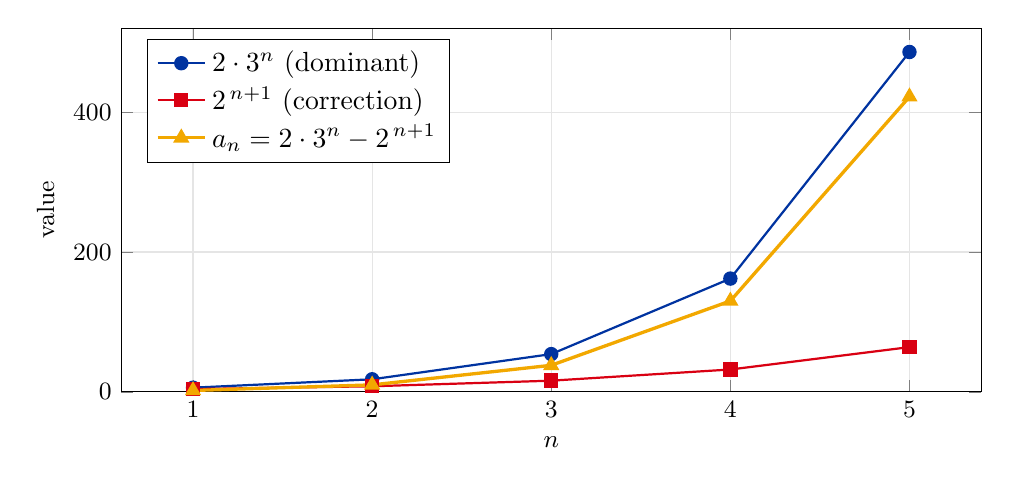
\begin{tikzpicture}
\begin{axis}[
  width=12.5cm, height=6.2cm,
  xlabel={$n$}, ylabel={value},
  xtick={1,2,3,4,5}, ymin=0, ymax=520,
  legend cell align=left, legend pos=north west,
  grid=both, grid style={gray!20},
  every axis plot/.append style={thick, mark size=2.2pt},
  tick label style={font=\small}, label style={font=\small}
]
\addplot[armBlue, mark=*] coordinates {(1,6)(2,18)(3,54)(4,162)(5,486)};
\addplot[armRed, mark=square*] coordinates {(1,4)(2,8)(3,16)(4,32)(5,64)};
\addplot[armOrange, very thick, mark=triangle*] coordinates {(1,2)(2,10)(3,38)(4,130)(5,422)};
\legend{$2\cdot3^n$ (dominant), $2^{\,n+1}$ (correction), $a_n=2\cdot3^n-2^{\,n+1}$}
\end{axis}
\end{tikzpicture}
\end{center}

\begin{center}
\small
\begin{tabular}{@{}c|cccccc@{}}
\toprule
$n$ & 1 & 2 & 3 & 4 & 5 & 6\\
\midrule
$a_n$ & 2 & 10 & 38 & 130 & 422 & 1330\\
$a_n/a_{n-1}$ & & $5$ & $3.80$ & $3.42$ & $3.25$ & $3.15$\\
\bottomrule
\end{tabular}
\end{center}

\smallskip
Look at the bottom row: the step-to-step growth rate $a_n/a_{n-1}$ is settling toward $3$,
the larger characteristic root. For large $n$ the $3^n$ term dwarfs the $2^{\,n+1}$ term, so
the sequence ends up growing almost exactly like $3^n$. This is the geometric guess paying
off in reverse: the roots we solved for really are the growth rates the recurrence was
hiding all along.

\begin{methodbox}
For a second-order linear homogeneous recurrence $a_n=p\,a_{n-1}+q\,a_{n-2}$:
\begin{enumerate}[leftmargin=1.5em,itemsep=1pt]
  \item Write the characteristic equation $r^2=pr+q$.
  \item \textbf{Two distinct roots} $r_1\neq r_2$: general solution $a_n=C r_1^n+D r_2^n$.
  \item \textbf{Repeated root} $r_1=r_2=r$: general solution $a_n=(C+Dn)\,r^n$
        (an extra factor $n$ - needed because $r^n$ alone gives only one solution).
  \item Find $C,D$ from the two initial values, then verify.
\end{enumerate}
\end{methodbox}

% =====================================================================
\section*{Problem 6 - Building a recurrence to count}

\begin{problembox}[6]
How many binary strings (strings of $0$s and $1$s) of length $10$ contain
\textbf{two consecutive zeros} (i.e.\ the block \textquotedbl{}$00$\textquotedbl{} appears somewhere)?
\end{problembox}

\begin{ideabox}
Counting strings that \emph{do} contain \textquotedbl{}$00$\textquotedbl{} directly is painful: the block can sit in
many overlapping places, and you would over-count strings that contain it more than once.

\textbf{Complementary counting.} It is far easier to count the \emph{opposite} -
strings with \textbf{no} \textquotedbl{}$00$\textquotedbl{} - and subtract from the total:
\[
\#(\text{contain }00) \;=\; \underbrace{2^{10}}_{\text{all strings}} \;-\; \#(\text{avoid }00).
\]
And \textquotedbl{}avoid $00$\textquotedbl{} is exactly the kind of property that builds up nicely one symbol at a
time - so it satisfies a recurrence.
\end{ideabox}

\textbf{Step 1 - Set up the count we actually want.}
Let
\[
f(n) = \#\{\text{binary strings of length } n \text{ with no two adjacent } 0\text{s}\}.
\]

\textbf{Step 2 - Find a recurrence by looking at the \emph{last} symbol.}
Take any \textquotedbl{}good\textquotedbl{} string of length $n$ and look at how it ends. There are exactly two
mutually exclusive cases, and each case is glued onto a shorter good string:

\begin{center}
\begin{tikzpicture}[
  font=\small, >=Stealth,
  blk/.style={draw, rounded corners=2pt, minimum height=8.5mm, align=center},
  bit/.style={draw, rounded corners=2pt, minimum height=8.5mm, minimum width=8mm}
]
% Case 1
\node[anchor=east] at (-0.3,0) {ends in \textbf{1}:};
\node[blk, minimum width=4.4cm, fill=armBlue!10] (g1) at (2.6,0)
  {good string of length $n-1$};
\node[bit, fill=armRed!15, right=1.2mm of g1] (one) {$1$};
\node[anchor=west] at ($(one.east)+(0.5,0)$) {$\rightarrow\ f(n-1)$ ways};

% Case 2
\node[anchor=east] at (-0.3,-1.5) {ends in \textbf{0}:};
\node[blk, minimum width=3.4cm, fill=armBlue!10] (g2) at (2.1,-1.5)
  {good string, length $n-2$};
\node[bit, fill=armRed!15, right=1.2mm of g2] (one2) {$1$};
\node[bit, fill=armOrange!25, right=1.2mm of one2] (zero2) {$0$};
\node[anchor=west] at ($(zero2.east)+(0.5,0)$) {$\rightarrow\ f(n-2)$ ways};
\node[font=\scriptsize\itshape, anchor=north, text=red!60!black] at (3.6,-2.05)
  {the symbol before a final $0$ must be $1$, otherwise we'd create \textquotedbl{}$00$\textquotedbl{}};
\end{tikzpicture}
\end{center}

\begin{itemize}[leftmargin=1.4em,itemsep=1pt]
  \item \textbf{Ends in $1$:} whatever comes before can be \emph{any} good string of length
        $n-1$ (adding a $1$ never creates \textquotedbl{}$00$\textquotedbl{}). That gives $f(n-1)$ strings.
  \item \textbf{Ends in $0$:} to avoid \textquotedbl{}$00$\textquotedbl{}, the symbol just before must be $1$, so the
        string ends in \textquotedbl{}$10$\textquotedbl{}. Whatever comes before is any good string of length $n-2$.
        That gives $f(n-2)$ strings.
\end{itemize}
The two cases never overlap and cover everything, so
\[
\boxed{\,f(n) = f(n-1) + f(n-2)\,}.
\]
This is the \textbf{Fibonacci rule} - counting reveals it on its own!

\textbf{Step 3 - Base cases (count tiny strings by hand).}
\[
\begin{aligned}
n=1:\ \{\,0,\ 1\,\} &\Rightarrow f(1)=2,\\
n=2:\ \{\,01,\ 10,\ 11\,\}\ (\text{not } 00) &\Rightarrow f(2)=3,\\
n=3:\ \{\,010,\ 011,\ 101,\ 110,\ 111\,\} &\Rightarrow f(3)=5.
\end{aligned}
\]
(Notice $5=3+2$, confirming the recurrence.)

\textbf{Step 4 - Run the recurrence up to $n=10$.}
\begin{center}
\small
\begin{tabular}{@{}c|cccccccccc@{}}
\toprule
$n$    & 1 & 2 & 3 & 4 & 5 & 6 & 7 & 8 & 9 & 10\\
\midrule
$f(n)$ & 2 & 3 & 5 & 8 & 13 & 21 & 34 & 55 & 89 & \textbf{144}\\
\bottomrule
\end{tabular}
\end{center}
So there are $f(10)=144$ length-$10$ strings that \emph{avoid} \textquotedbl{}$00$\textquotedbl{}.

\textbf{Step 5 - Complementary count.}
\[
\#(\text{contain } 00) = 2^{10} - f(10) = 1024 - 144 = 880.
\]

\answer{$880$ binary strings of length $10$ contain two consecutive zeros.}

\begin{methodbox}
\textbf{Two transferable tricks here:}
\begin{enumerate}[leftmargin=1.5em,itemsep=1pt]
  \item \emph{Complementary counting} - when \textquotedbl{}at least one bad pattern\textquotedbl{} is messy, count the
        clean strings and subtract from the total.
  \item \emph{Last-symbol case split} - to build a recurrence for strings with a local
        forbidden pattern, branch on how the string ends; each branch attaches a fixed
        suffix to a shorter valid string.
\end{enumerate}
\end{methodbox}

\end{document}
